% 一线三等角（K 字型）：水平直线 l 上三点 A、P、B
% 同侧（上方）有 C、D，使 ∠CAP = ∠CPD = ∠DBP = α
% 由对称构造（α=60°）：A=(-3,0), B=(3,0), P=(0,0), C=(-1.5,2.598), D=(1.5,2.598)
\documentclass[tikz,border=4pt]{standalone}
\usepackage{ctex}
\usepackage{amsmath}
\usetikzlibrary{calc}
\begin{document}
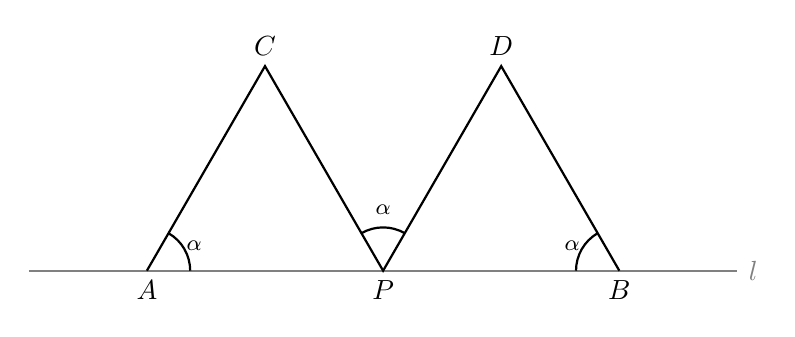
\begin{tikzpicture}[scale=1.0, thick]
  \draw[gray] (-4.5, 0) -- (4.5, 0);
  \node[gray] at (4.7, 0) {$l$};

  \coordinate (A) at (-3, 0);
  \coordinate (P) at (0, 0);
  \coordinate (B) at (3, 0);
  \coordinate (C) at (-1.5, 2.598);
  \coordinate (D) at (1.5, 2.598);

  \draw (A) -- (C) -- (P) -- (D) -- (B);

  % 角 ∠CAP（A 点，AB 方向到 AC 方向，60°）
  \draw ($(A) + (0.55, 0)$) arc[start angle=0, end angle=60, radius=0.55];
  \node at (-2.4, 0.32) {\footnotesize $\alpha$};

  % 角 ∠CPD（P 点，PD 方向 60° 到 PC 方向 120°）
  \draw ($(P) + ({0.55*cos(60)}, {0.55*sin(60)})$)
        arc[start angle=60, end angle=120, radius=0.55];
  \node at (0, 0.78) {\footnotesize $\alpha$};

  % 角 ∠DBP（B 点，BA 方向 180° 到 BD 方向 120°）
  \draw ($(B) + (-0.55, 0)$) arc[start angle=180, end angle=120, radius=0.55];
  \node at (2.4, 0.32) {\footnotesize $\alpha$};

  \node[below] at (A) {$A$};
  \node[below] at (P) {$P$};
  \node[below] at (B) {$B$};
  \node[above] at (C) {$C$};
  \node[above] at (D) {$D$};
\end{tikzpicture}
\end{document}
